\documentclass{beamer}
\usepackage{../371g-slides}
% Uncomment these lines to print notes pages
% \pgfpagesuselayout{4 on 1}[letterpaper,border shrink=5mm,landscape]
% \setbeameroption{show only notes}
\title{Simple regression}
\subtitle{Lecture 2}
\author{STA 371G}

\begin{document}
  

  \frame{\maketitle}

  % Show outline at beginning of each section
  \AtBeginSection[]{
    \begin{frame}<beamer>
      \tableofcontents[currentsection]
    \end{frame}
  }

  %%%%%%% Slides start here %%%%%%%

  \begin{darkframes}
    \begin{frame}{About the course staff}
      \begin{itemize}
        \item Instructor: \textbf{Brian Lukoff, Ph.D.}
          \begin{itemize}
            \item Office hours: M/W 11 AM-12 PM in CBA 3.440
            \item Contact: \texttt{brian.lukoff@utexas.edu} or 415-652-8853
          \end{itemize}
        \item TAs:
          \begin{itemize}
            \item Office hours: M 11:30 AM-1:30 PM, 2-4 PM, W 12-2 PM, Th 4-6 PM in CBA 4.304
            \item Help session: T 6-7 PM in the ModLab
          \end{itemize}

          \vspace{0.2in}
          \begin{center}
            \begin{tabular}{ccc}
              
\includegraphics[width=1.1in]{vasko} &
              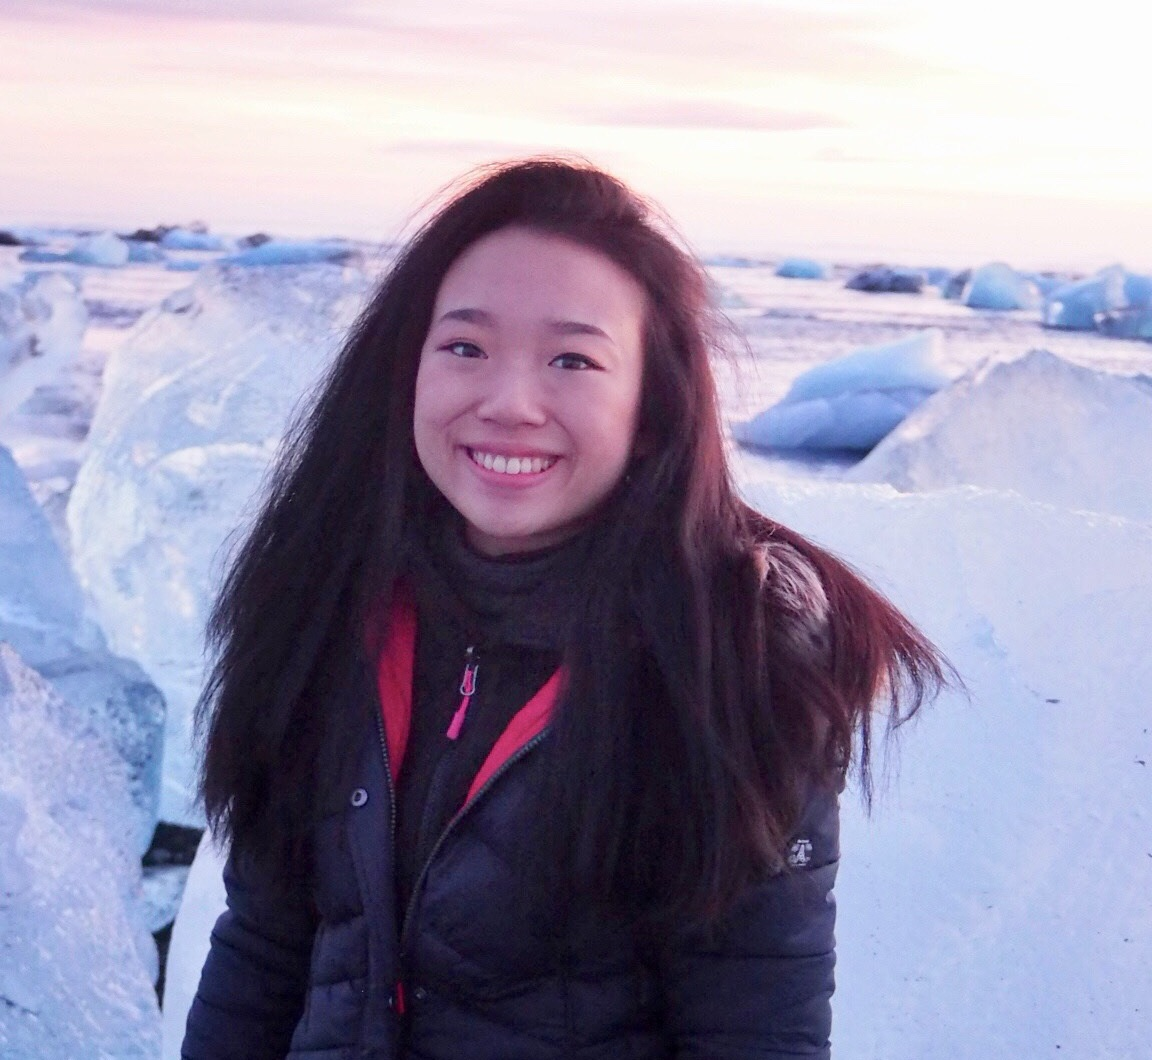
\includegraphics[width=1.1in]{nicole} &
              
\includegraphics[width=1.1in]{zameer} \\
              Vasko Lalkov & Nicole Chia & Zameer Vaswani \\
            \end{tabular}
          \end{center}
      \end{itemize}
    \end{frame}

    \begin{frame}
      \begin{center}
        
\includegraphics[width=3in]{add-health}

        \bigskip
        National Longitudinal Study of Adolescent to Adult Health

        \bigskip
        Nationally representative sample of US students in grades 7-12 were surveyed in the 1994-95 school year (\url{http://www.cpc.unc.edu/projects/addhealth})

        \bigskip
        Students were followed up on with subsequent in-home interviews four times (most recently 2008)
      \end{center}
    \end{frame}

    \begin{frame}
      This is an \textbf{awesome} data set, with data on:
      \begin{columns}[onlytextwidth]
        \column{.5\textwidth}
          \begin{itemize}
            \item family
            \item relationships
            \item health
            \item military service
            \item religion
            \item sex and STDs
            \item economics
            \item education
          \end{itemize}
        \column{.5\textwidth}
          \begin{itemize}
            \item personality
            \item criminality
            \item tobacco
            \item drugs
            \item alcohol
            \item pregnancy
            \item sleep
            \item daily activities
          \end{itemize}
      \end{columns}
    \end{frame}

    \begin{frame}
      \begin{center}
        Do people that start drinking younger tend to drink more (or less) when they become adults?
      \end{center}
      \bigskip\pause
      We want to know:
      \begin{itemize}[<+->]
        \item What is our best \textbf{prediction} of alcohol consumption if we know at what age had their first drink?
        \item How good is that prediction?
        \item What is the \textbf{relationship} between alcohol consumption and age of first drink?
      \end{itemize}
    \end{frame}

    \begin{frame}
      \begin{tabular}{ll}
        Age of first drink & \textbf{Predictor variable} \\
        Number of drinks consumed as adult & \textbf{Response variable} \\
      \end{tabular}
    \end{frame}

    \begin{frame}[fragile]
      \note{
        Point out R command and syntax. \textCR
        Ask what's wrong with this? \textCR
        Introduce the idea of a codebook here.
      }
\begin{knitrout}
\definecolor{shadecolor}{rgb}{0.137, 0.137, 0.137}\begin{kframe}
\begin{alltt}
\hlstd{> }\hlkwd{hist}\hlstd{(addhealth4}\hlopt{$}\hlstd{h4to34,}
\hlstd{+ }  \hlkwc{main}\hlstd{=}\hlstr{''}\hlstd{,} \hlkwc{xlab}\hlstd{=}\hlstr{'Age of first drink'}\hlstd{,}
\hlstd{+ }  \hlkwc{col}\hlstd{=}\hlstr{'orange'}\hlstd{)}
\end{alltt}


{\ttfamily\noindent\bfseries\color{errorcolor}{Error in hist(addhealth4\$h4to34, main = "{}"{}, xlab = "{}Age of first drink"{}, : object 'addhealth4' not found}}\end{kframe}
\end{knitrout}
      \lc
    \end{frame}

    \begin{frame}{Let's examine our variables}
      \begin{center}
        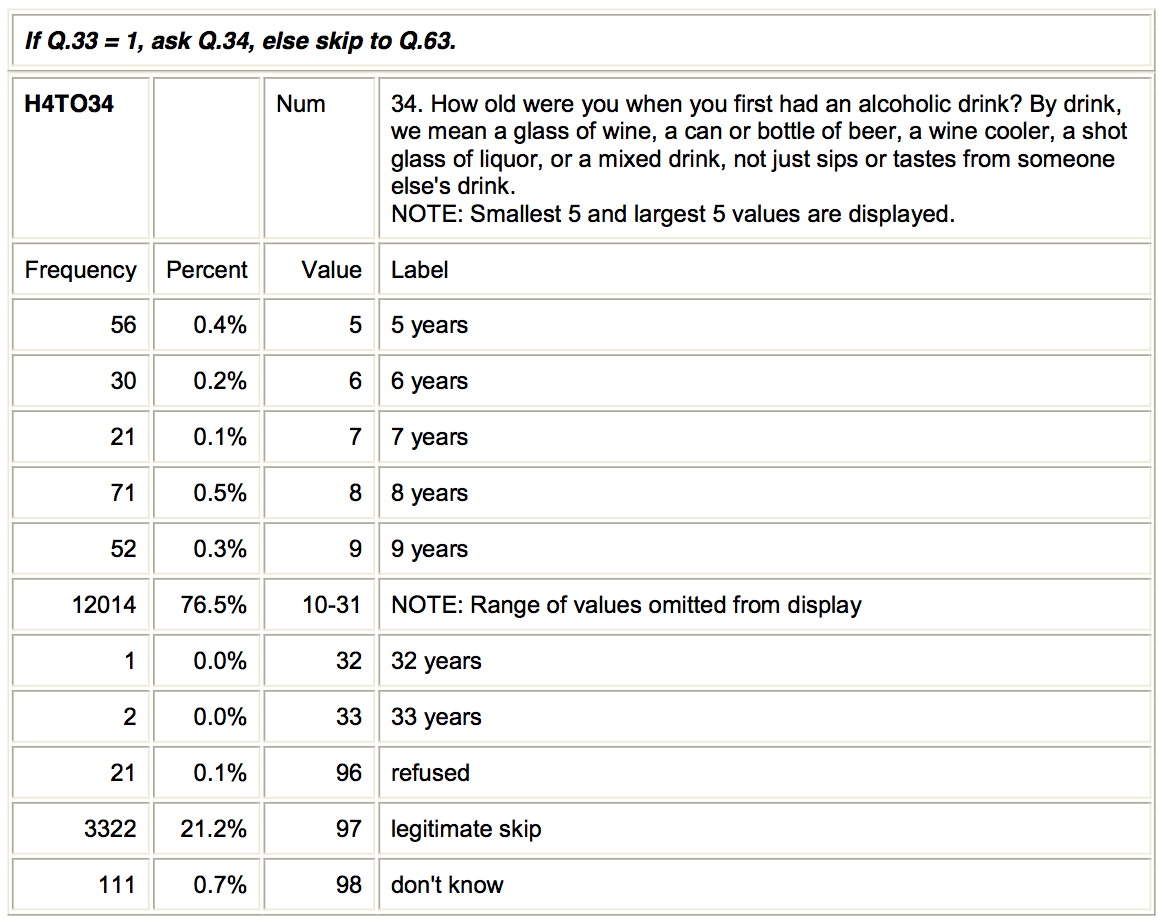
\includegraphics[width=3.5in]{h4to34_codebook.png}
      \end{center}
    \end{frame}

    \begin{frame}[fragile]
\begin{knitrout}
\definecolor{shadecolor}{rgb}{0.137, 0.137, 0.137}\begin{kframe}
\begin{alltt}
\hlstd{> }\hlstd{age} \hlkwb{<-} \hlstd{addhealth4}\hlopt{$}\hlstd{h4to34}
\end{alltt}


{\ttfamily\noindent\bfseries\color{errorcolor}{Error in eval(expr, envir, enclos): object 'addhealth4' not found}}\begin{alltt}
\hlstd{> }\hlstd{age[age} \hlopt{>=} \hlnum{96}\hlstd{]} \hlkwb{<-} \hlnum{NA}
\end{alltt}


{\ttfamily\noindent\bfseries\color{errorcolor}{Error in age[age >= 96] <- NA: object 'age' not found}}\begin{alltt}
\hlstd{> }\hlkwd{hist}\hlstd{(age,} \hlkwc{main}\hlstd{=}\hlstr{''}\hlstd{,} \hlkwc{xlab}\hlstd{=}\hlstr{''}\hlstd{,} \hlkwc{col}\hlstd{=}\hlstr{'orange'}\hlstd{)}
\end{alltt}


{\ttfamily\noindent\bfseries\color{errorcolor}{Error in hist(age, main = "{}"{}, xlab = "{}"{}, col = "{}orange"{}): object 'age' not found}}\end{kframe}
\end{knitrout}
    \end{frame}

    \begin{frame}{Let's examine our variables}
      \begin{center}
        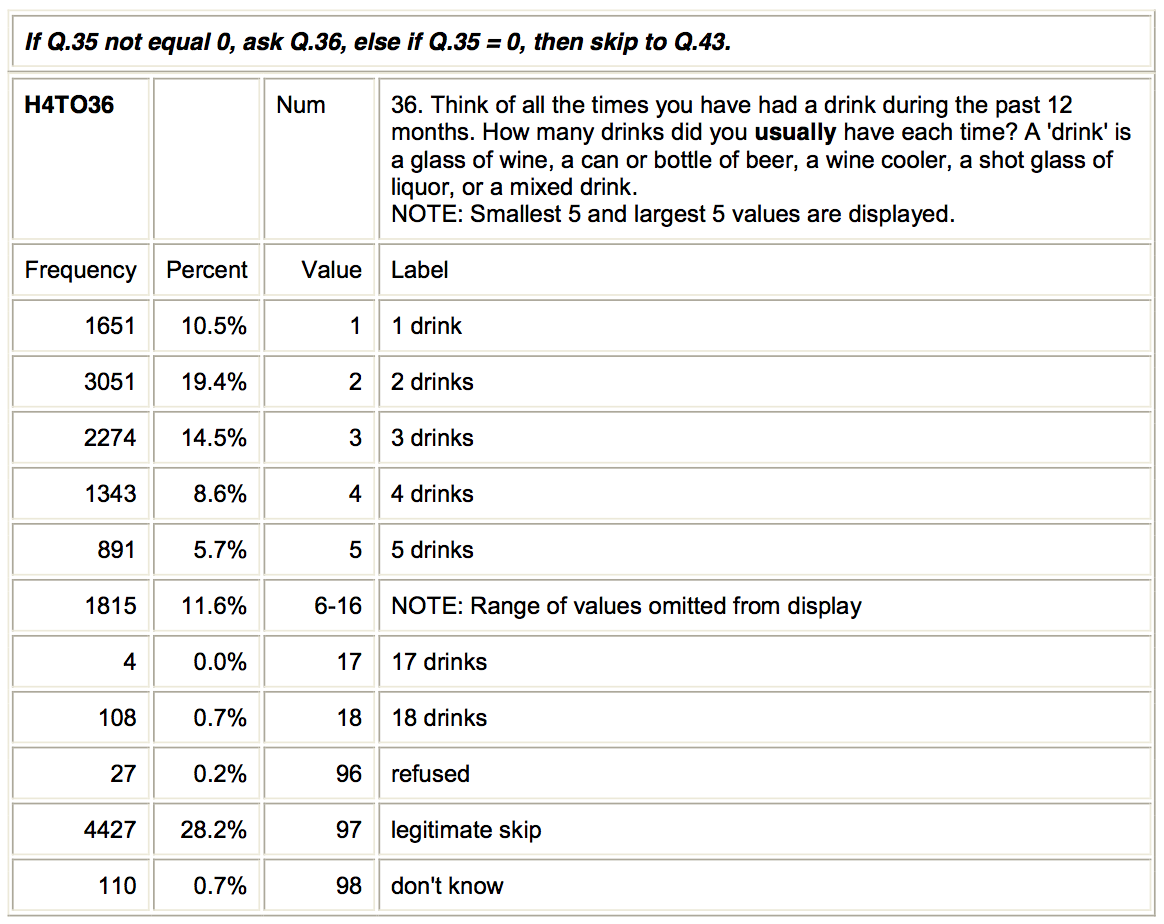
\includegraphics[width=3.5in]{h4to36_codebook.png}
      \end{center}
    \end{frame}

    \begin{frame}[fragile]
\begin{knitrout}
\definecolor{shadecolor}{rgb}{0.137, 0.137, 0.137}\begin{kframe}
\begin{alltt}
\hlstd{> }\hlstd{num.drinks} \hlkwb{<-} \hlstd{addhealth4}\hlopt{$}\hlstd{h4to36}
\end{alltt}


{\ttfamily\noindent\bfseries\color{errorcolor}{Error in eval(expr, envir, enclos): object 'addhealth4' not found}}\begin{alltt}
\hlstd{> }\hlstd{num.drinks[num.drinks} \hlopt{>=} \hlnum{96}\hlstd{]} \hlkwb{<-} \hlnum{NA}
\end{alltt}


{\ttfamily\noindent\bfseries\color{errorcolor}{Error in num.drinks[num.drinks >= 96] <- NA: object 'num.drinks' not found}}\begin{alltt}
\hlstd{> }\hlkwd{hist}\hlstd{(num.drinks,} \hlkwc{main}\hlstd{=}\hlstr{''}\hlstd{,} \hlkwc{xlab}\hlstd{=}\hlstr{'How many drinks'}\hlstd{,}
\hlstd{+ }  \hlkwc{col}\hlstd{=}\hlstr{'orange'}\hlstd{)}
\end{alltt}


{\ttfamily\noindent\bfseries\color{errorcolor}{Error in hist(num.drinks, main = "{}"{}, xlab = "{}How many drinks"{}, col = "{}orange"{}): object 'num.drinks' not found}}\end{kframe}
\end{knitrout}
    \end{frame}


    \begin{frame}[fragile]
\begin{knitrout}
\definecolor{shadecolor}{rgb}{0.137, 0.137, 0.137}\begin{kframe}
\begin{alltt}
\hlstd{> }\hlkwd{plot}\hlstd{(num.drinks} \hlopt{~} \hlstd{age,} \hlkwc{pch}\hlstd{=}\hlnum{16}\hlstd{,} \hlkwc{col}\hlstd{=}\hlstr{'orange'}\hlstd{,}
\hlstd{+ }  \hlkwc{xlab}\hlstd{=}\hlstr{'Age of first drink'}\hlstd{,}
\hlstd{+ }  \hlkwc{ylab}\hlstd{=}\hlstr{'Number of drinks consumed'}\hlstd{)}
\end{alltt}


{\ttfamily\noindent\bfseries\color{errorcolor}{Error in eval(predvars, data, env): object 'num.drinks' not found}}\end{kframe}
\end{knitrout}
    \end{frame}

    \begin{frame}[fragile]
\begin{knitrout}
\definecolor{shadecolor}{rgb}{0.137, 0.137, 0.137}\begin{kframe}
\begin{alltt}
\hlstd{> }\hlkwd{plot}\hlstd{(}\hlkwd{jitter}\hlstd{(num.drinks,} \hlnum{4}\hlstd{)} \hlopt{~} \hlkwd{jitter}\hlstd{(age,} \hlnum{4}\hlstd{),}
\hlstd{+ }  \hlkwc{pch}\hlstd{=}\hlnum{46}\hlstd{,} \hlkwc{col}\hlstd{=}\hlstr{'orange'}\hlstd{,}
\hlstd{+ }  \hlkwc{xlab}\hlstd{=}\hlstr{'Age of first drink'}\hlstd{,}
\hlstd{+ }  \hlkwc{ylab}\hlstd{=}\hlstr{'Number of drinks consumed'}\hlstd{)}
\end{alltt}


{\ttfamily\noindent\bfseries\color{errorcolor}{Error in jitter(num.drinks, 4): object 'num.drinks' not found}}\end{kframe}
\end{knitrout}
    \end{frame}

    \begin{frame}[fragile]
      The regression line is the line of ``best fit'' through this plot:
\begin{knitrout}
\definecolor{shadecolor}{rgb}{0.137, 0.137, 0.137}\begin{kframe}


{\ttfamily\noindent\bfseries\color{errorcolor}{Error in eval(predvars, data, env): object 'num.drinks' not found}}

{\ttfamily\noindent\bfseries\color{errorcolor}{Error in eval(predvars, data, env): object 'num.drinks' not found}}

{\ttfamily\noindent\bfseries\color{errorcolor}{Error in abline(model, col = "{}red"{}, lwd = 4): object 'model' not found}}\end{kframe}
\end{knitrout}
      \lc
    \end{frame}

    \begin{frame}{What is linear regression doing?}
      We model each case ($x_i=$ age for $i$th person, $y_i=$ number of drinks for $i$th person) as a linear relationship plus some error:
      \[
        y_i = \beta_0 + \beta_1 x_i + \epsilon_i
      \]
      $\beta_0$ and $\beta_1$ are the intercept and slope, respectively.
      \bigskip\pause

      We find estimates for $\beta_0$ and $\beta_1$ in our sample that \emph{minimize} the errors:
      \[
        \hat Y = \hat\beta_0 + \hat\beta_1 X
      \]
      This is the regression (best fit) line.
    \end{frame}

    \begin{frame}[fragile]
      \fontsize{9}{9}\selectfont
\begin{knitrout}
\definecolor{shadecolor}{rgb}{0.137, 0.137, 0.137}\begin{kframe}
\begin{alltt}
\hlstd{> }\hlstd{model} \hlkwb{<-} \hlkwd{lm}\hlstd{(num.drinks} \hlopt{~} \hlstd{age)}
\end{alltt}


{\ttfamily\noindent\bfseries\color{errorcolor}{Error in eval(predvars, data, env): object 'num.drinks' not found}}\begin{alltt}
\hlstd{> }\hlkwd{summary}\hlstd{(model)}
\end{alltt}


{\ttfamily\noindent\bfseries\color{errorcolor}{Error in summary(model): object 'model' not found}}\end{kframe}
\end{knitrout}
      \lc
    \end{frame}

    \begin{frame}[fragile]
      This translates to a regression line of:
\begin{knitrout}
\definecolor{shadecolor}{rgb}{0.137, 0.137, 0.137}\begin{kframe}


{\ttfamily\noindent\bfseries\color{errorcolor}{Error in eval(expr, envir, enclos): object 'model' not found}}

{\ttfamily\noindent\bfseries\color{errorcolor}{Error in eval(expr, envir, enclos): object 'model' not found}}

{\ttfamily\noindent\bfseries\color{errorcolor}{Error in summary(model): object 'model' not found}}

{\ttfamily\noindent\bfseries\color{errorcolor}{Error in summary(model): object 'model' not found}}\end{kframe}
\end{knitrout}





